\documentclass[10pt]{homework}
\usepackage[utf8]{inputenc}
\usepackage{amsmath}
\usepackage{amssymb,amsthm}
\usepackage{braket}
\usepackage{mathrsfs}
\usepackage{physics}
\usepackage{enumitem}
\usepackage{verbatim}
\usepackage[pdfpagelabels]{hyperref}
\usepackage{xcolor}
\usepackage{tabularx}
\usepackage{framed}
\usepackage{float}
\usepackage{graphicx}
\usepackage{subcaption}
\usepackage{color}
\usepackage{listings}
\definecolor{customgreen}{rgb}{0,0.6,0}
\definecolor{customgray}{rgb}{0.5,0.5,0.5}
\definecolor{custommauve}{rgb}{0.6,0,0.8}
\lstset{language=Go,
  basicstyle=\ttfamily\scriptsize,
  keywordstyle=\color{blue}\ttfamily,
  stringstyle=\color{red}\ttfamily,
  commentstyle=\color{customgreen}\ttfamily}

% CHANGE THE FOLLOW THREE LINES!
\newcommand{\hwname}{Ruiying Ma, Zhengyuan Su, Haofeng Huang}
\newcommand{\hwnum}{2-1}

\DeclareMathOperator*{\maximize}{maximize}
\DeclareMathOperator*{\argmin}{argmin}
\DeclareMathOperator*{\minimize}{minimize}
\DeclareMathOperator*{\subjectto}{subject\;to}
\DeclareMathOperator*{\vect}{vec} \DeclareMathOperator*{\mat}{mat}
\DeclareMathOperator*{\diag}{diag}
\newcommand{\J}{\mathcal{J}}
\newcommand{\I}{\mathcal{I}}
\definecolor{lightgray}{gray}{0.95} % 10%

\newenvironment{packed_enumerate}{
\begin{enumerate}
  \setlength{\itemsep}{1pt}
  \setlength{\parskip}{0pt}
  \setlength{\parsep}{0pt}
}{\end{enumerate}}

\newenvironment{packed_itemize}{
\begin{itemize}
  \setlength{\itemsep}{1pt}
  \setlength{\parskip}{0pt}
  \setlength{\parsep}{0pt}
}{\end{itemize}}


% CHANGE THESE ONLY ONCE PER CLASS
\newcommand{\hwtype}{Project Report}
\newcommand{\hwclass}{Operating Systems and Distributed Systems 2023}
\newcommand{\hwclasssimplified}{OS and DS 2023}

\begin{document}

\hypersetup{pageanchor=false}
\maketitle
\hypersetup{pageanchor=true}
\pagenumbering{arabic}

\section{\textbf{Assumption}}

We assume that we have a perfect network. There is no netowrk failure and all messages will be received eventually.

\section{\textbf{Design}}

We implement a decentralized blockchain network with 5 miner machines and 5 client processes. 

\subsection*{Wallet}


\begin{lstlisting}
  type Wallet struct {
    SK []byte // secret key
    PK []byte // public key
    Address	[]byte // address
  }
\end{lstlisting}

A wallet is equivalent to a user in the blockchain network. A real-world person can create multiple wallets. A wallet has a \textit{public key} and a \textit{secret key}. With the public key, the \textit{address} of this wallet can be computed using a specific hash function. Once a wallet is created, the public key and the address of this wallet are broadcast to the network. A created wallet is stored offline.




\subsection*{Transaction}

\begin{lstlisting}
  type In struct {
    HashTx	[]byte  // this income is gained from this tx
    Idx	int // this income is gained from this payment
    Amount	int   // the amount of this income
  }

  type Out struct {
    Amount	int  // the amount of this payment
    Recipient	[]byte // the address of the recipient
  }

  type Transaction struct {
    Initiator	[]byte  // the public key of the initiator of this transaction
    Incomes		[]In  // the incomes this transaction contains
    Payments	[]Out  // the payments this transaction contrains
    IsReward 	bool  // whether this transaction is a reward of block mining
    Hash		[]byte  // the hash of this transaction
    Signature	[]byte  // the signature of this transaction by the initiator
  }
\end{lstlisting}

A transaction is first signed and then hashed. The hash serves as an abstract of this transaction. When we want to identify this transaction, we only need to use its hash. Hashing is performed after signing so that different transactions (including the reward transactions) have different hashes.

When verifying a transaction, we check
\begin{itemize}
  \item Whether the transaction's incomes are valid (unspent, belongs to initiator). No need to check this for reward transaction.
  \item Whether the transaction's payments are valid. That is, payments $\leq$ incomes.
  \item Whether the transaction's signature is valid.
  \item Whether the transaction's hash is valid.
\end{itemize}

\subsection*{Block}

\begin{lstlisting}
  type Block struct {
    Txs	[]*Transaction  // set of transactions this block contains
    TxHashes	[]byte  // the hash of all the transactions
    PrevHash 	[]byte  // the hash of the previous block
    Time 	int64  // the time when this block is created
    Nonce 	int
    Height 	int  // the position of this block in the blockchain (count from 0)
    IsGenisis	bool  // whether this block is the genisis block (the first block of the blockchain)
    Hash 	[]byte  // the hash of this block
  }
\end{lstlisting}

When verifying a block, we check
\begin{itemize}
  \item Whether the block's \texttt{TxHashes} is correct.
  \item Whether there is at most one reward transaction in this block.
  \item Whether the block's previous hash is correct. No need to check this for the genesis block. 
  \item Whether the block's height is correct.
  \item Whether the block's transactions are all legitimate.
  \item Whether the block's nonce is legitimate.
  \item Whether the block's hash is correct.
\end{itemize}

Notice that when a miner is going to make a block from a set of transactions, it should ensure that a transaction initiator can only occur once in this block. This aims to defend double-spent attack.

\subsection*{Blockchain}

\begin{lstlisting}
  type BlockChain struct {
    DB	*bolt.DB  // the offline database that stores the blockchain
  }
\end{lstlisting}

The blockchain is stored in the offline database of each machine. We implement a 1-confirmation blockchain (i.e., when branch occurs, if a branch is longer by 1 block, then this branch is chosen). 

When appending a block \texttt{B} to the blockchain, we 
\begin{itemize}
  \item Check whether this block is legitimate.
  \item If the block is legitimate, we update the blockchain using Nakamoto's rules. Suppose the highest block in the blockchain is \texttt{B'}. Whether \texttt{B} will be  appended to the blockchain is determined by the following process:
  \begin{itemize}
    \item If \texttt{B.Height} $<$ \texttt{B'.Height}, then \texttt{B} won't be appended to the blockchain.
    \item If \texttt{B.Height} $=$ \texttt{B'.Height}, then \texttt{B} will be appended to the blockchain if \texttt{B} is created before \texttt{B'}, that is, \texttt{B.Time} $<$ \texttt{B'.Time}.
  \end{itemize}
\end{itemize}


\subsection*{Network Layout}

We implement a decentralized network. The network consists of 5 miners. Each miner can
\begin{itemize}
  \item broadcast a transaction (can consider this functionality as a client process)
  \item mine and broadcast a block
  \item receive and handle a transaction
  \item receive and handle a block
\end{itemize}

\begin{lstlisting}
  type Miner struct {
    BC        *blockchain.BlockChain  // the blockchain of this miner
    MID       string  // the machine id of this miner
    Mempool   map[string]blockchain.Transaction  // the memory pool that stores transactions received by this miner
    Addrs     map[string][]string  // the addresses of all the peers in the network
    bc_lock   chan bool  // the lock of the blockchain
    mem_lock  chan bool  // the lock of the memory pool
    addr_lock chan bool  // the lock of the address map
  }
\end{lstlisting}

At first all miners create their wallets and broacast the public keys and addresses. Each miner stores the addresses and public keys of other miners. 

Then, a designated miner will create the genisis block and get the reward. This miner then distributes this reward evenly to all other miners to ensure that all miners have some money before they being to generate transactions.

Now, all miners begin to generate transactions, mine blocks, and handle messages. When a miner receives a transaction, it adds this transaction to its memory pool. If there are sufficiently many transactions in the memory pool, the miner begins to generate a block. Once the block is generated, the miner will broadcast it to all peers. When a miner receives a block, it will check the validity of this block and append the legitimate block to its blockchain.

When handling messages, each miner should make sure that there is no concurrency issue when accessing \texttt{Addrs}, \texttt{Mempool} and its blockchain \texttt{BC}.

\section{\textbf{Evaluations and Results}}

We evaluate the disitribution of the time to mine a block. We also evaluate the distribution of the time to verify the validity of a block. 

\begin{itemize}
  \item Time to mine a block
  \begin{figure}[htbp]
    \centering
    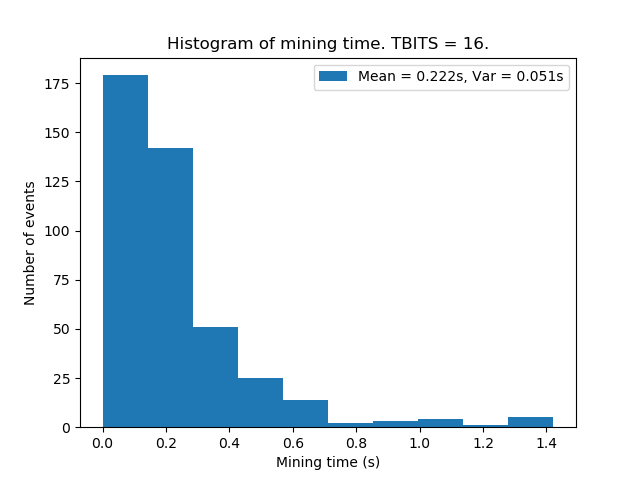
\includegraphics[scale = 0.8]{../plot/mining_time_16.png}
  \end{figure}

  We can see that the distribution is consistent with the one we've seen in class.
  \item Time to verify a block
  \begin{figure}[htbp]
    \centering
    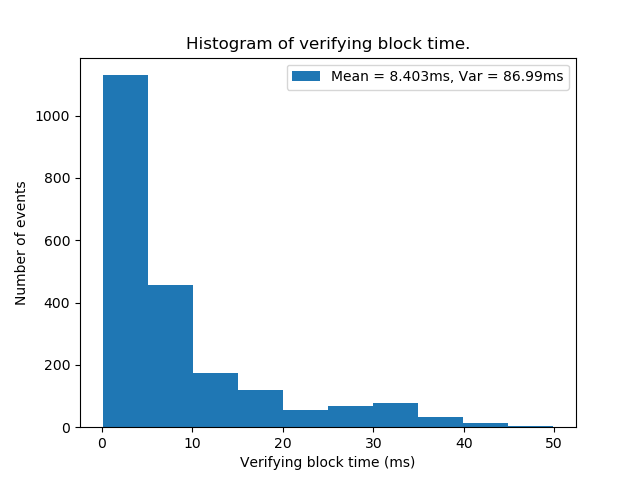
\includegraphics[scale = 0.8]{../plot/verifying_block_time.png}
  \end{figure}
\end{itemize}

\section{\textbf{Improvement Proposal}}

We may implement the following features/improvements later:
\begin{itemize}
  \item A Merkle tree for transactions in the same block
  \item A UTXO set to speedup block/transaction verifaction
  \item $k$-Confirmation with $k$ greater than one
  \item Dynamically adjust the difficulty of POW
  \item Allow a user to create a wallet at any time and use it in the future (i.e., a p2p network such that a user can join/leave dynamically)
\end{itemize}

\section{\textbf{References}}

We referred to \href{https://github.com/Jeiwan/blockchain_go/tree/master}{a centralized blockchain implementation} and \href{https://pkg.go.dev/github.com/boltdb/bolt}{the Bolt DB documents}.


\end{document}